
%
%  $Description: Author guidelines and sample document in LaTeX 2.09$ 
%
%  $Author: ienne $
%  $Date: 1995/09/15 15:20:59 $
%  $Revision: 1.4 $
%

\documentclass[10pt,twocolumn]{article} 
\usepackage{latex8}
\usepackage{listings}
\usepackage{graphicx}

%\documentstyle[times,art10,twocolumn,latex8]{article}

%------------------------------------------------------------------------- 
% take the % away on next line to produce the final camera-ready version 
\pagestyle{empty}

\newcommand{\url}[1]{\textsf{#1}}
\newcommand{\code}[1]{\lstinline{#1}}
\newcommand{\csharp}{C{\normalfont \#}}
\newcommand{\comment}[1]{}
\newcommand\codefamily\sffamily
\lstset{language={[Sharp]C},mathescape=true,flexiblecolumns=true,morekeywords={alloc,delay,delete,expose,let,unsatisfiable,receive,rep,contract,message,state,one},basicstyle=\codefamily\small,literate={->}{{$\rightarrow$}}{2}{<<}{{$\langle$}}{2}{>>}{{$\rangle$}}{2}{!}{{\textbf{!}}}{2},frame=lines,moredelim=[is][\itshape]{@}{@},captionpos=b,numberstyle=\tiny,stepnumber=1,numbersep=2pt}

%------------------------------------------------------------------------- 
\begin{document}

\title{Exploiting the Synergy between Automated-Test-Generation and Programming-by-Contract} 

\author{Mike Barnett, Manuel F\"ahndrich, Peli de Halleux, Francesco Logozzo, and Nikolai Tillmann\\
Microsoft Research, One Microsoft Way, Redmond, WA, 98052-6399, USA\\
{\tt \{mbarnett, maf, jhalleux, logozzo, nikolait\}@microsoft.com}\\
}

\maketitle
\thispagestyle{empty}

\begin{abstract}
This demonstration presents two tools, Code Contracts and Pex, that utilize specification
constructs for advanced testing, runtime checking, and static checking
of object-oriented .NET programs. 
\end{abstract}
\vspace*{-5mm}

%------------------------------------------------------------------------- 
\Section{Introduction}
Over the last few years we have been working on influencing the way programmers
develop .NET software through two related projects: Code Contracts and Pex.
{\em Code Contracts} provides a specification technique for expressing
method pre- and postconditions as well as object invariants.
These specifications are then used for runtime checking and static
checking.
The specifications are also understood by the advanced unit-testing
tool, Pex.
{\em Pex} 
performs a white box code analysis using a constraint solver to determine relevant test inputs.
Preconditions allow pruning of irrelevant test inputs, and
postconditions guide test generation and allow detecting bugs;
object invariants serve both purposes.
Furthermore, Pex enables the concept of Parameterized Unit Tests
which are essentially parameterized usage scenarios 
annotated with specifications to state assumptions and assertions.
The result of Pex's analysis is a small unit test suite which often achieves high code coverage.

Both tools can be invoked through the command-line, 
and they integrate with Microsoft Visual Studio through add-ins. 
%------------------------------------------------------------------------- 
\Section{Specification Language}
We are targeting the specification language and tools at the general
developer, not the verification enthusiast.
It is thus important to
use a single form of specifications that meets three
simultaneous goals:
\begin{enumerate}
\item Specifications serve as documentation. They must be as
  readable as possible.
\item Specifications should be executable. This
  motivates writing specifications for testing and immediate perceived
  benefit, without consideration of static verification.
\item Specifications simplify static verification.
\end{enumerate}
Our specification approach is language-agnostic: we use
idiomatic code written in the developer's source language to express
them. 
\begin{figure}[thb]
\begin{small}
\begin{lstlisting}
int Increment(int value, string label) {
  Contract.Requires( value > 0 );
  Contract.Requires( label != null );
  Contract.Ensures( Count == 
                    Contract.OldValue(Count) + value );
  Contract.Ensures( Contract.Result<int>()
                    == Contract.OldValue(Count) );
  ...
\end{lstlisting}
\caption{An Increment specification in \csharp}
\label{fig:csharp}
\end{small}
\end{figure}
Preconditions and postconditions are expressed as calls to the static
methods \lstinline{Contract.Requires} and
\lstinline{Contract.Ensures}. Special dummy methods are used to refer
to the method's return value as well as referring to the \emph{old}
value of an expression, meaning the value of the expression on method
entry. The conditions in the example in Figure~\ref{fig:csharp} are written in \csharp{}
expression syntax.

A language-agnostic approach has many advantages: 
\begin{itemize}
\item Developers need not learn a new language for
specifications. Predicates are boolean conditions expressed in the
source language.
\item No new front-ends or compilers are required. Standard compilers directly translate contracts into
  .NET intermediate language (MSIL). As a benefit, compilers
  check the syntax and typing of contract conditions, thus avoiding errors in specifications,
  such as unresolved names, that would arise if the specifications
  were written in comments or attributes.
\item Standard development environments help writing
  specifications in the same way they help writing other code, via highlighting, intellisense,
  completion, etc.
\item The semantics of contracts is defined by that the semantics of the generated MSIL. 
  The compiled code acts as a persisted format of specifications consumable by a variety of tools.
\end{itemize}
The language independence extends from the specification language to
the tools themselves as they consume the
generated MSIL rather than on the source.

%------------------------------------------------------------------------- 
\Section{Runtime Contract Checking}
In a post-build step, the compiled binaries containing the calls to the contract
methods are transformed by having each specification injected at the 
appropriate program points.
For instance, method postconditions are moved to the exit points of each method
and calls to Contract.Result are replaced with the return value of the method.
At the beginning of each method, arguments to Contract.OldValue are evaluated and
stored into locals which then replace those method calls within the postcondition-checking
code.

In addition, contracts from supertypes and interfaces are inherited by subtypes
and interface implementations. This provides the basis for enforcing behavioral
subtyping \cite{Liskov-Wing94}, which is required for modular checking.

%------------------------------------------------------------------------- 
\Section{Static Checking}
Our static checker is based on abstract interpretation rather than
SMT solvers traditionally used for program verification, in order to
automate the generation of loop
invariants and strongest postconditions.

Although we use modular verification which, in principle, requires
specifications at all method boundaries, we use techniques to infer
pre- and postconditions whenever possible.

The existing abstract domains provide an analysis that checks for
null dereferences, array indexing, arithmetic overflow, in addition
to user-defined general properties.

%------------------------------------------------------------------------- 
\Section{Test Generation}
Pex~\cite{pex} is an automatic white-box test generation tool for .NET.
Starting from a designated method,
Pex explores the statements of all transitively reachable callees
using 
\emph{dynamic symbolic execution}~\cite{godefroid05:dart}.
% This technique consists in executing a designated entry point method,
% starting with very simple inputs,
% while performing a symbolic execution in parallel to collect symbolic constraints on inputs
% obtained from predicates in branch statements along the execution.
Pex uses a constraint solver to compute 
% variations of the previous inputs
test inputs that exercise particular program paths.
% in order to steer future program executions along different execution paths.
Pex employs heuristic search strategies to select 
% path variations
paths 
that are likely to 
be feasible and
exhibit different program behaviors.
As a result, 
Pex often finds relevant test inputs quickly and fully automatically,
while still exercising all feasible execution paths eventually.

When trying to 
% change a previous path, 
determine relevant execution paths,
Pex considers explicit conditional branch statements
as well all operations that can cause exceptional control flow changes as a side effect.
Furthermore, Pex leverages preconditions, postconditions, and object invariants as follows.
The compiled binaries are transformed by a post-build step as described earlier,
so that all specifications are injected. 
This results in additional conditional program branches 
which distinguish the case when the specification holds from the case where it does not hold.
As a result, Pex will try to exercise both cases during its program analysis.
When test inputs cause a top-level precondition or object invariant violation,
these test inputs are discarded and are not shown to the user.
In all other cases of specification violations, the result is a test case that is flagged as a failure.

% Pex uses the SMT solver Z3~\cite{bjorner07:Z3} to reason about the feasibility of variations of previous execution paths,
% and to obtain ground models for constraint systems.
% As the number of potential variations explodes with the number of branches in the program,
% Pex uses various search strategies that have been highly effective, see e.g.~\cite{fitness}.
% As a result, Pex code analysis requires only little user input.

The analysis produces a set of unit tests,
saved in a file as source code.
Each test sets up particular test input, and then calls the entry point method.
Pex can be configured to support the unit test idioms of various unit testing frameworks,
including NUnit~\cite{nunit} and MSTest~\cite{mstest}.

\Section{Parameterized Unit Testing}

A parameterized unit test (PUT) is
simply a method that takes parameters,
states assumptions on the arguments,
performs a sequence of method calls that exercise the code-under-test,
and asserts properties of the code's expected behavior.
PUTs are a generalization of traditional unit tests.
While preconditions, postconditions, and object invariants can only express
specifications that must hold at method boundaries,
PUTs allow to express properties that span multiple method calls.

%------------------------------------------------------------------------- 
\Section{Synergies}
We already touched upon how runtime checked contracts improve
automated test generation by providing more assumptions and test
outcomes. A drawback of static checking is the
presence of false warnings and the effort to determine whether a
warning is warranted or not. Pex often helps alleviate this problem by
being able to point out inputs to a method that actually trigger the
violation. Pex reports the issues as source code that can be debugged
immediately by the developer. Furthermore, Pex can suggest new preconditions at
appropriate places to avoid problems it finds, thereby strengthening
the specifications and closing the cycle.
%------------------------------------------------------------------------- 
%------------------------------------------------------------------------- 
\comment{
\Section{Tool Status}
Both Code Contracts and Pex are available for commercial use through 
DevLabs, a site used for early evaluation of potential technologies from
Microsoft.

Future work includes producing formatted documentation from the specifications.
}
%------------------------------------------------------------------------- 

\begin{figure*}[tb]
\begin{center}
  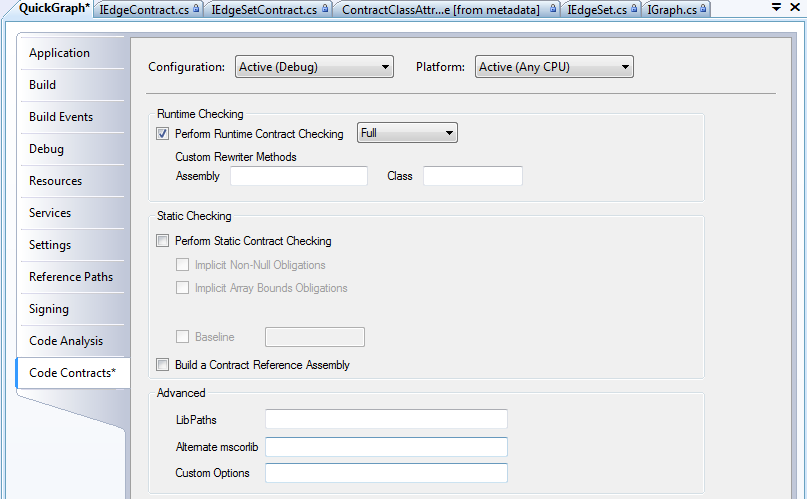
\includegraphics[width=2\columnwidth]{ContractUI.png}
\end{center}
\caption{The Code Contact User Interface}
\label{fig:contractui}
\end{figure*}

\begin{figure*}[tb]
\begin{center}
  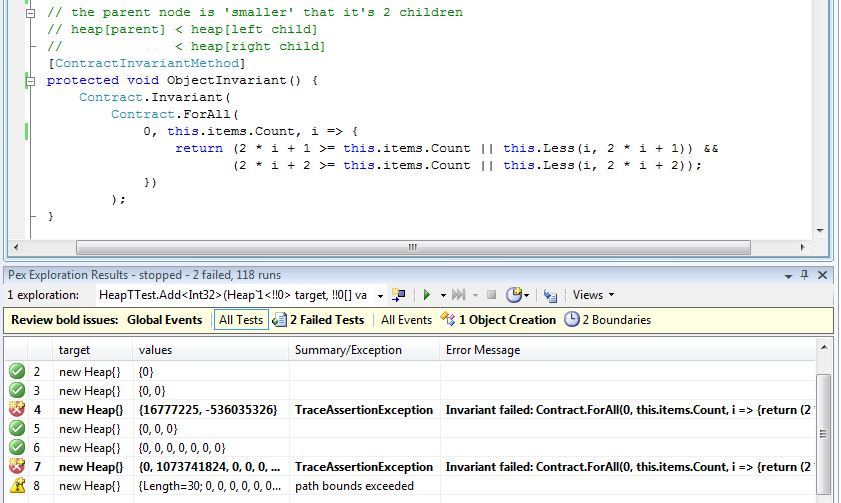
\includegraphics[width=2\columnwidth]{pexscreenshot.png}
\end{center}
\caption{Screenshot of Pex Output}
\label{fig:pexoutput}
\end{figure*}

\section{Demonstration Description}
The demonstration will consist of a tag-team talk between a member of
the code contract team and a member of the Pex team. During the
demonstration, we will live author code and run the static analysis
tool, which will point out errors. We will use Pex to find counter
examples that exhibit the erroneous behavior. To guard against these
errors, we will author more contracts, in
particular object invariants. Running our tools again, will find more places
where the code is either incomplete or wrong and we will author live
fixes. We also show how Pex is used to obtain a series of unit tests
that provide very high-coverage of the module being developed.

\begin{figure}[thb]
\begin{small}
\begin{lstlisting}
Function Increment(ByVal value As Integer) As Integer
  Contract.Requires( value > 0 )
  Contract.Requires( label IsNot Nothing )
  Contract.Ensures( Count
                    = Contract.OldValue(Count) + value )
  Contract.Ensures( Contract.Result(Of Integer)()
                    = Contract.OldValue(Count) )
  ...
\end{lstlisting}
\end{small}
\caption{An Increment specification in Visual Basic}
\label{fig:vb}
\end{figure}

\section{Screenshots}
Figure~\ref{fig:contractui} shows the contract user interface in
Visual Studio. The UI allows the programmer to enable runtime checking
and/or static checking. The integration in the IDE manages all the
extra build steps transparently.

As an example of the language-agnostic approach, the same
specification as in Figure~\ref{fig:csharp} can be written in Visual
Basic as shown in Figure~\ref{fig:vb}.

Figure~\ref{fig:pexoutput} shows the output of Pex during test
generation. Test entries in the list on the left marked green are
succeeding tests, while red ones are failing tests. Test number 4
found an input that violated the invariant of a binary heap.


\begin{figure}[htb]
\begin{center}
  \includegraphics[width=\columnwidth]{FoxtrotOutput.png}
\end{center}
\caption{Example of Runtime Contract Failure}
\label{fig:foxtrot}
\end{figure}

\begin{figure*}[tb]
\begin{center}
  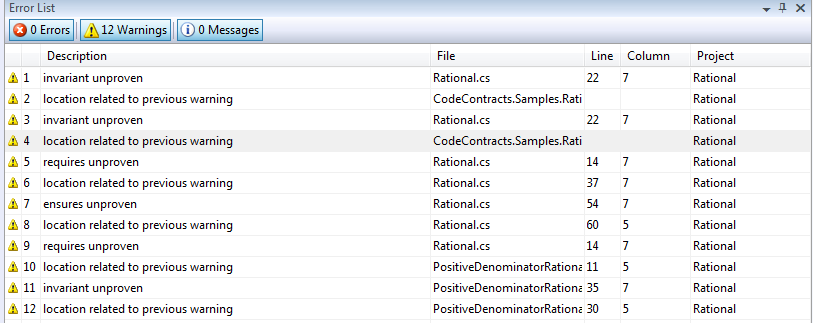
\includegraphics[width=2\columnwidth]{staticCheckerOutput.png}
\end{center}
\caption{Example of Static Checker Output}
\label{fig:clousot}
\end{figure*}

Figure~\ref{fig:foxtrot} shows the default contract failure behavior
when runtime checking of contracts is enabled. In this case, an
invariant was violated.

Figure~\ref{fig:clousot} shows the output produced by a run of the
static contract verifier.


\bibliographystyle{latex8}
\bibliography{bib}

\end{document}

